\documentclass[12pt]{article}

\usepackage{graphicx}
\graphicspath{{../Fichier_Image}}

\title{Hypothèse 3.(a) Porte Bureaux Milieu}
\author{Thibault Clodion}

\begin{document}

\maketitle % Permet d'afficher le titre, l'author etc
 
Attention : ne pas oublier que l'on a montré qu'il fallait pas que les bureaux est enormement de portes : 11 premiers bâtiments
\newline\newline
\underline{Hypothèse :} Les bureaux du milieux (s'ils sont assez grand (3.(b))) ont besoin de plusieurs portes pour diminuer le temps de sorties
\newline\newline
\underline{Expérience :} Une expérience où les bureaux du mileux ont qu'une porte et une où ils en ont deux (avec 8. et 5. des 10 premiers bâtiment)
\newline\newline

On considera que les bureaux du milieux sont ceux dans la zone entourée en rouge (environ).
\newline\newline
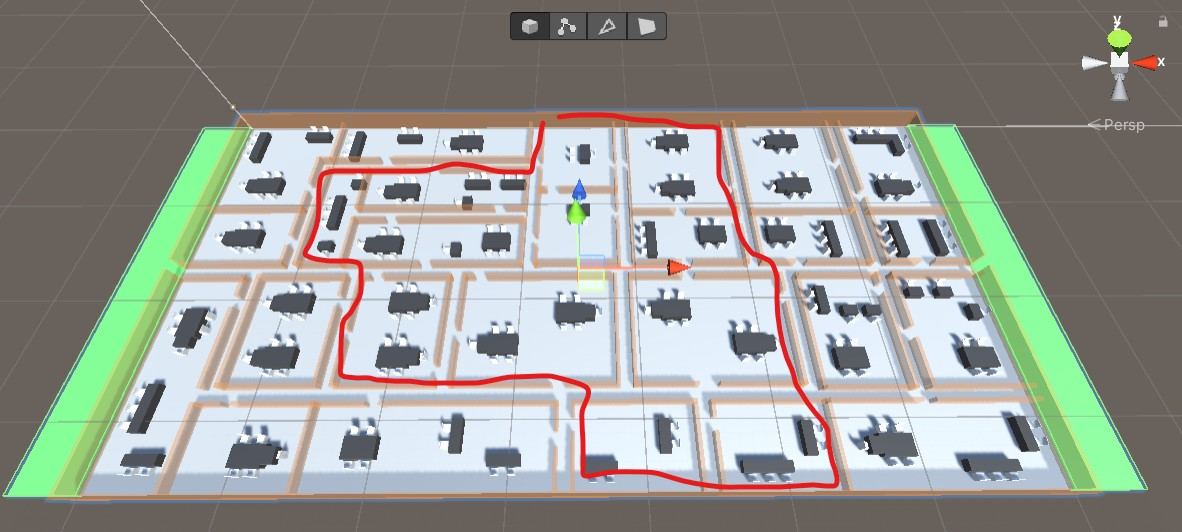
\includegraphics[scale=0.5]{3.(a) Porte bureaux milieux .jpg}
\newline\newline

3.(a) 5. avec 1 porte
\newline\newline
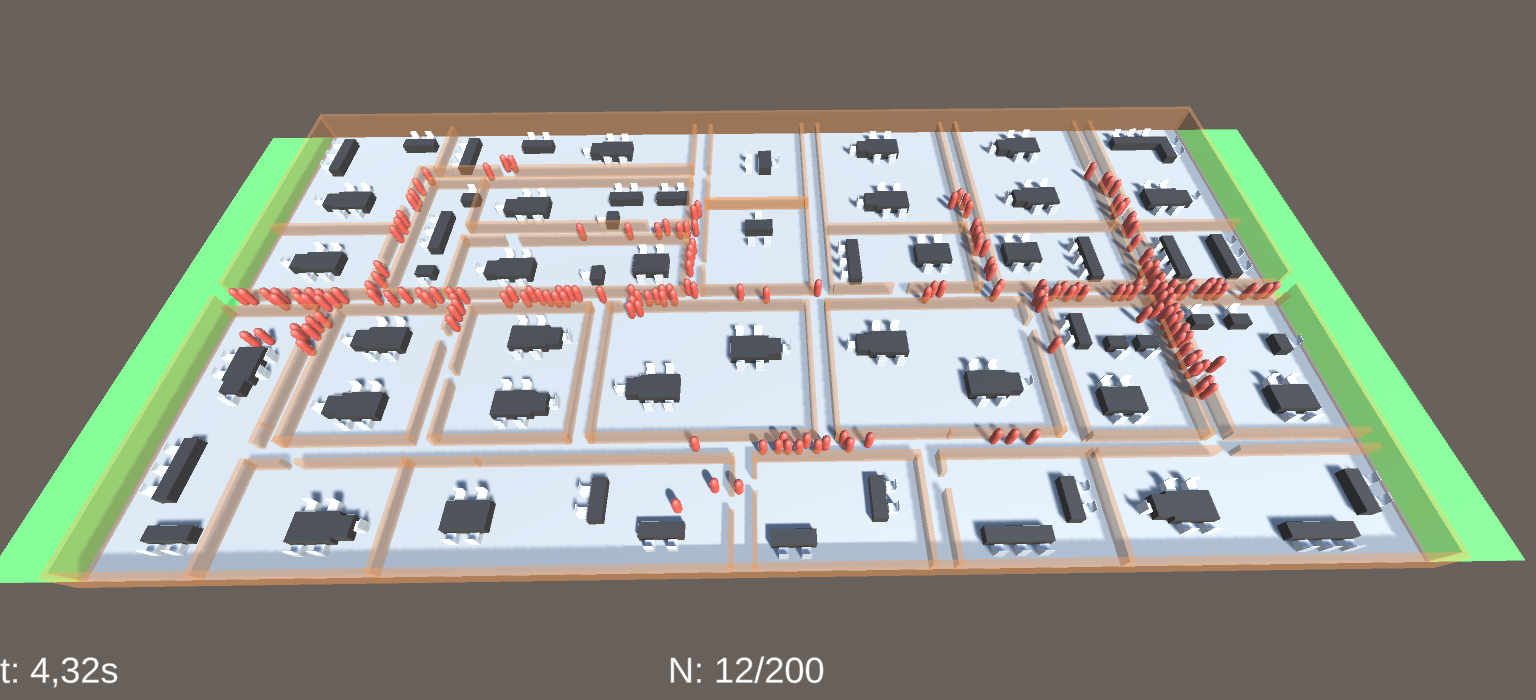
\includegraphics[scale=0.3]{3.(a) 5. avec 1 porte.png}
\newline\newline
Temps moyen de dernière sortie : 24.89s
\newline
$\hspace*{0.2cm}$- Certains prennent du temps pour sortir (comme ceux en bas) car ils doivent uniquement passé par des couloirs et donc leur chemin est rallongé comparé à quand les bureaux
du milieu servent de passage.
\newline
$\hspace*{0.2cm}$- Le trafic est plutôt fluide comme chaque bureaux amenne à un couloir différent et qu'il ne rentre pas dans d'autre bureaux. (efficace pour réguler le flux)
\newline\newline

3.(a) 5. avec 2 portes
\newline\newline
Temps moyen de dernière sortie : 22.74s
\newline
$\hspace*{0.2cm}$- Certains nouveaux chemins sont empruntés mais le changement est minime
\newline
$\hspace*{0.2cm}$- Finalement cela rajoute peut-être plus de flux à voir avec les temps.
\newline\newline

3.(a) 5. avec 3 portes
\newline\newline
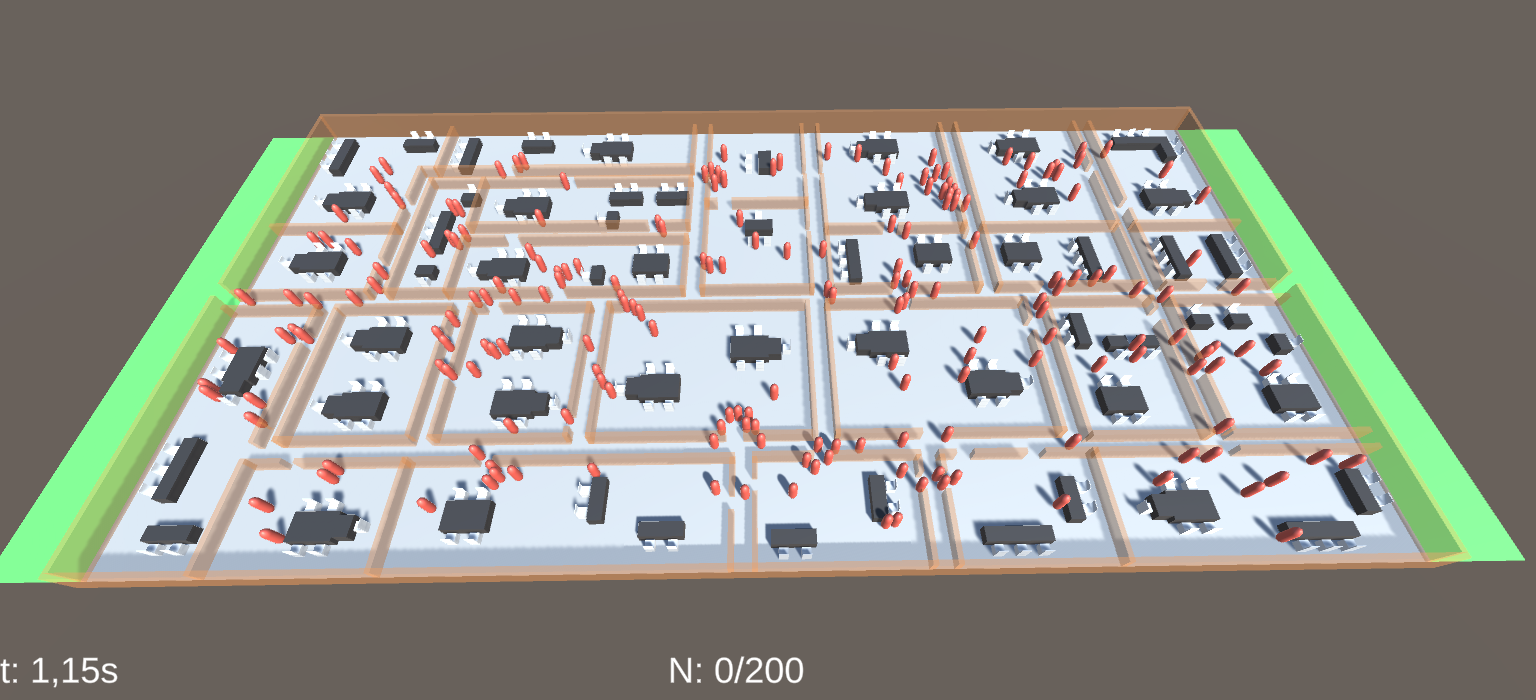
\includegraphics[scale=0.3]{3.(a) 5. avec 3 porte.png}
\newline\newline
Temps moyen de dernière sortie : 22.80s
\newline
$\hspace*{0.2cm}$- On voit que de nouveaux chemins se sont créés mais les gens empruntent plutôt les couloirs car c'est plus rapide.
\newline
$\hspace*{0.2cm}$-
\newline\newline

3.(a) 8. avec 1 porte
\newline\newline
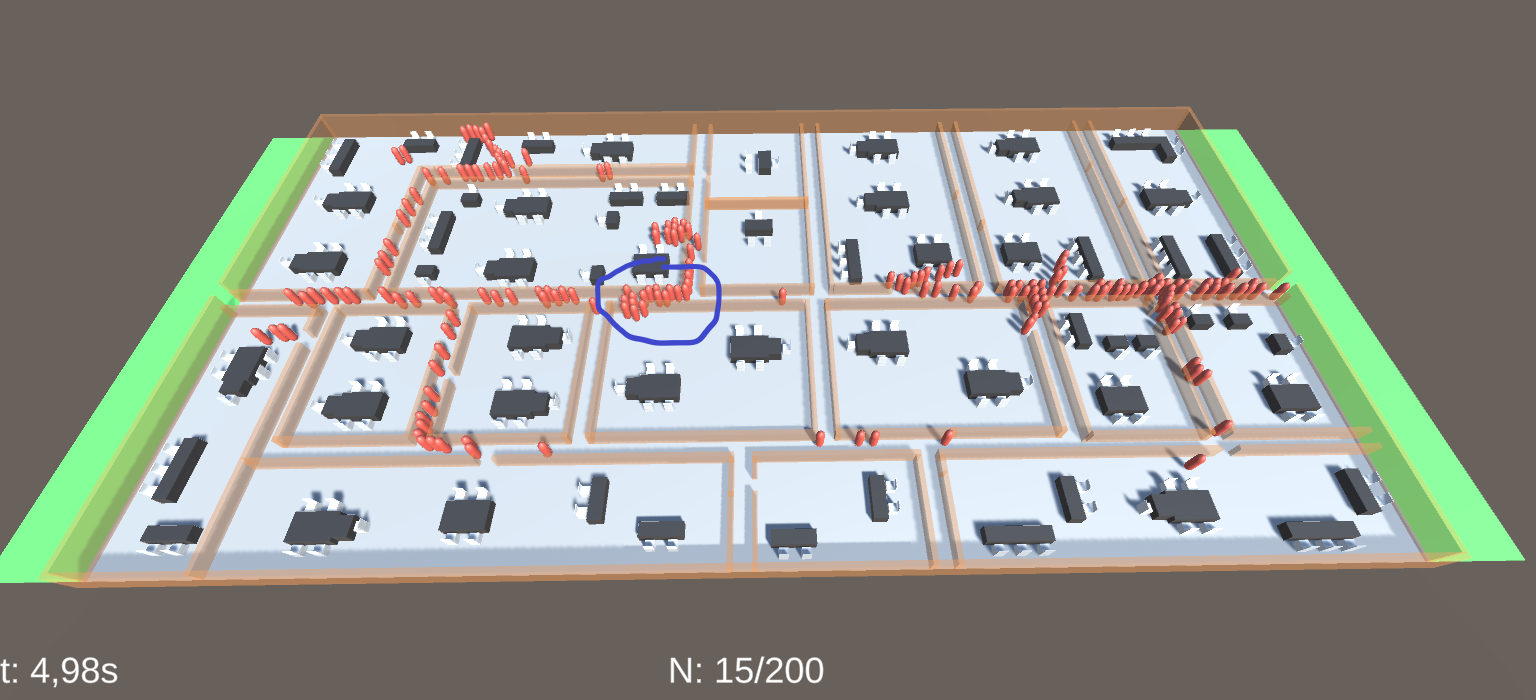
\includegraphics[scale=0.3]{3.(a) 8. avec 1 porte.png}
\newline\newline
Temps moyen de dernière sortie : 27.37s
\newline
$\hspace*{0.2cm}$- Tout le monde emprunte les même couloirs (unicité du chemin presque)
\newline
$\hspace*{0.2cm}$- Certains quitte un bureau et tente d'aller à droite et d'autre à gauche, cela créer des collisions et donc des ralentissement (deux flux opossés)
\newline\newline

3.(a) 8. avec 2 portes
\newline\newline
Temps moyen de dernière sortie : 21.76s
\newline
$\hspace*{0.2cm}$- Plus de chemins différent emprunté
\newline
$\hspace*{0.2cm}$- Une arrivé plus rapide vers la sortie qui provoque des poussements
\newline\newline

3.(a) 8. avec 3 portes
\newline\newline
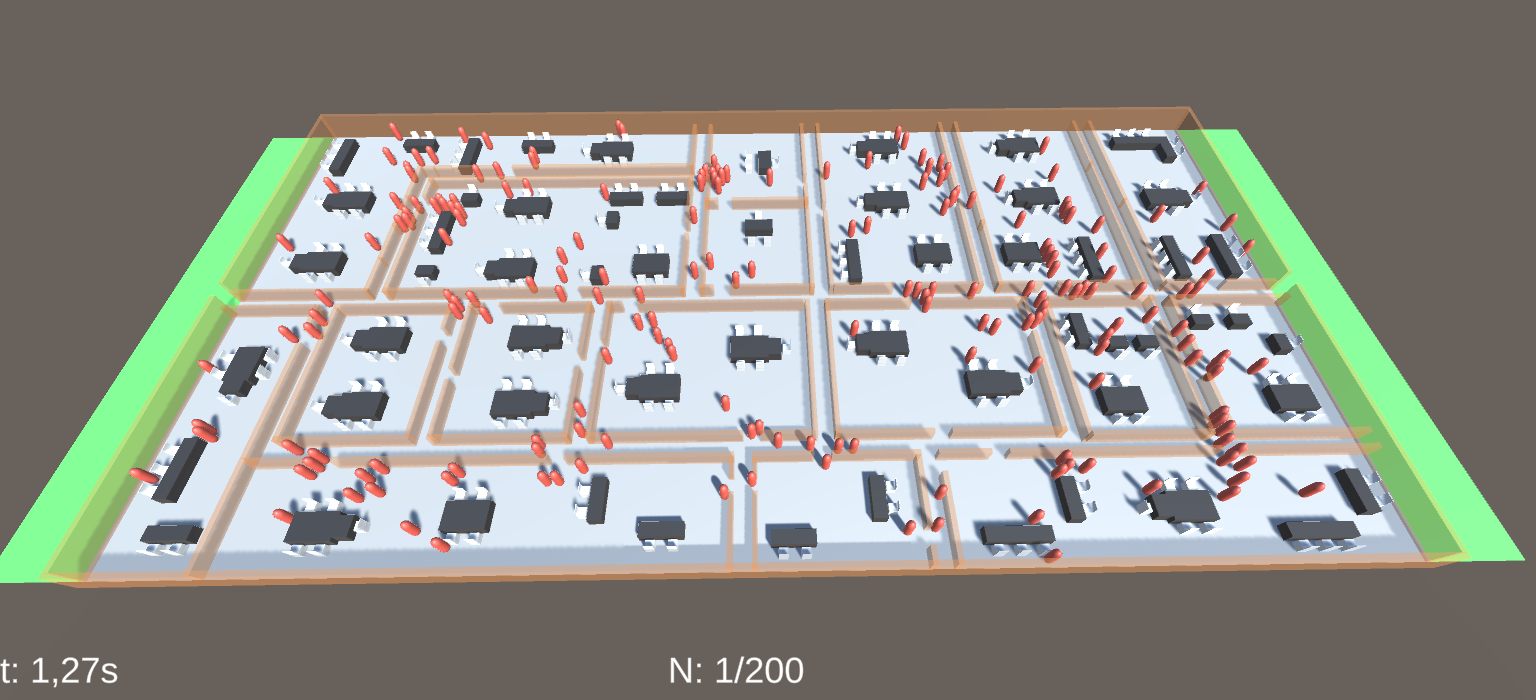
\includegraphics[scale=0.3]{3.(a) 8. avec 3 portes.png}
\newline\newline
Temps moyen de dernière sortie : 21.95s
\newline
$\hspace*{0.2cm}$- La sortie des bureaux est plus rapide, et l'accès vers la sortie également.
\newline
$\hspace*{0.2cm}$- Il y a beaucoup de monde qui arrive proche des sorties vite.
\newline\newline

\section{Resultat du 5. avec 1,2 ou 3 portes}
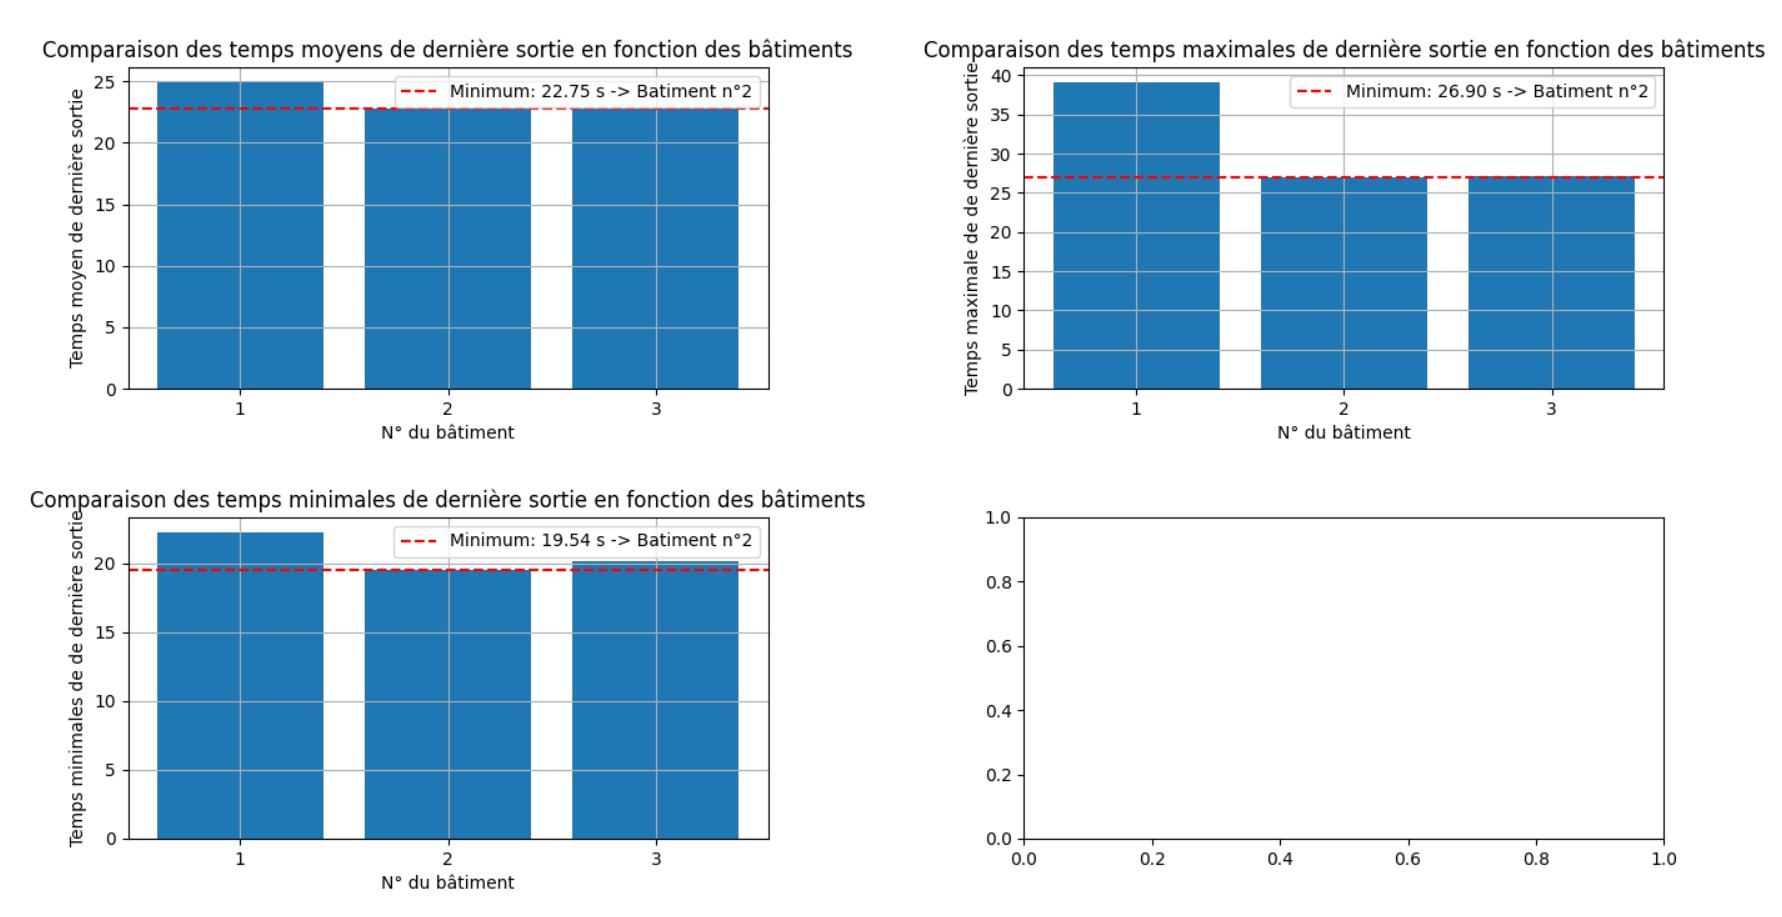
\includegraphics[scale=0.4]{3.(a) Resultat 5.jpg}
\newline\newline

Les résultats sont très cohérent avec l'hypothèse faite, 2 portes fais en effet diminuer le temps et 3 portes le fait légèrement augmenter
(ce qui s'explique car on ne veut pas créer unicité du chemin emprunté (le plus court))


\section{Resultat 8. avec 1,2 ou 3 portes}
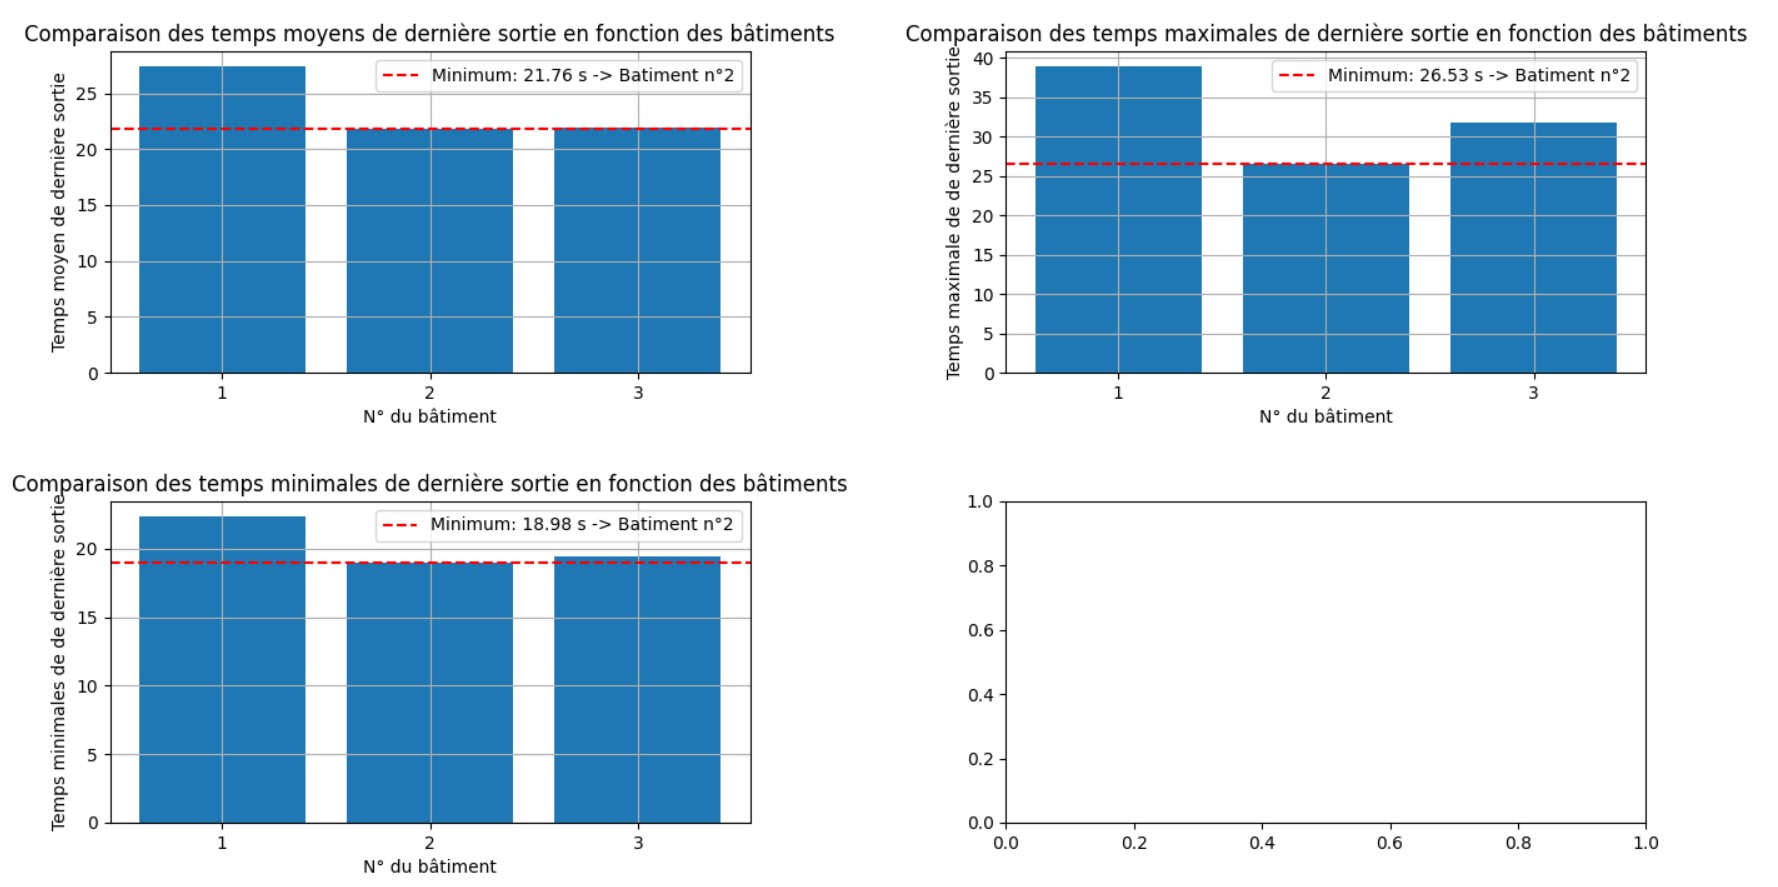
\includegraphics[scale=0.4]{3.(a) Resultat 8.jpg}
\newline\newline

On retrouve exactement les mêmes conclusions que pour le batiment 5.

\section{Resultat final}
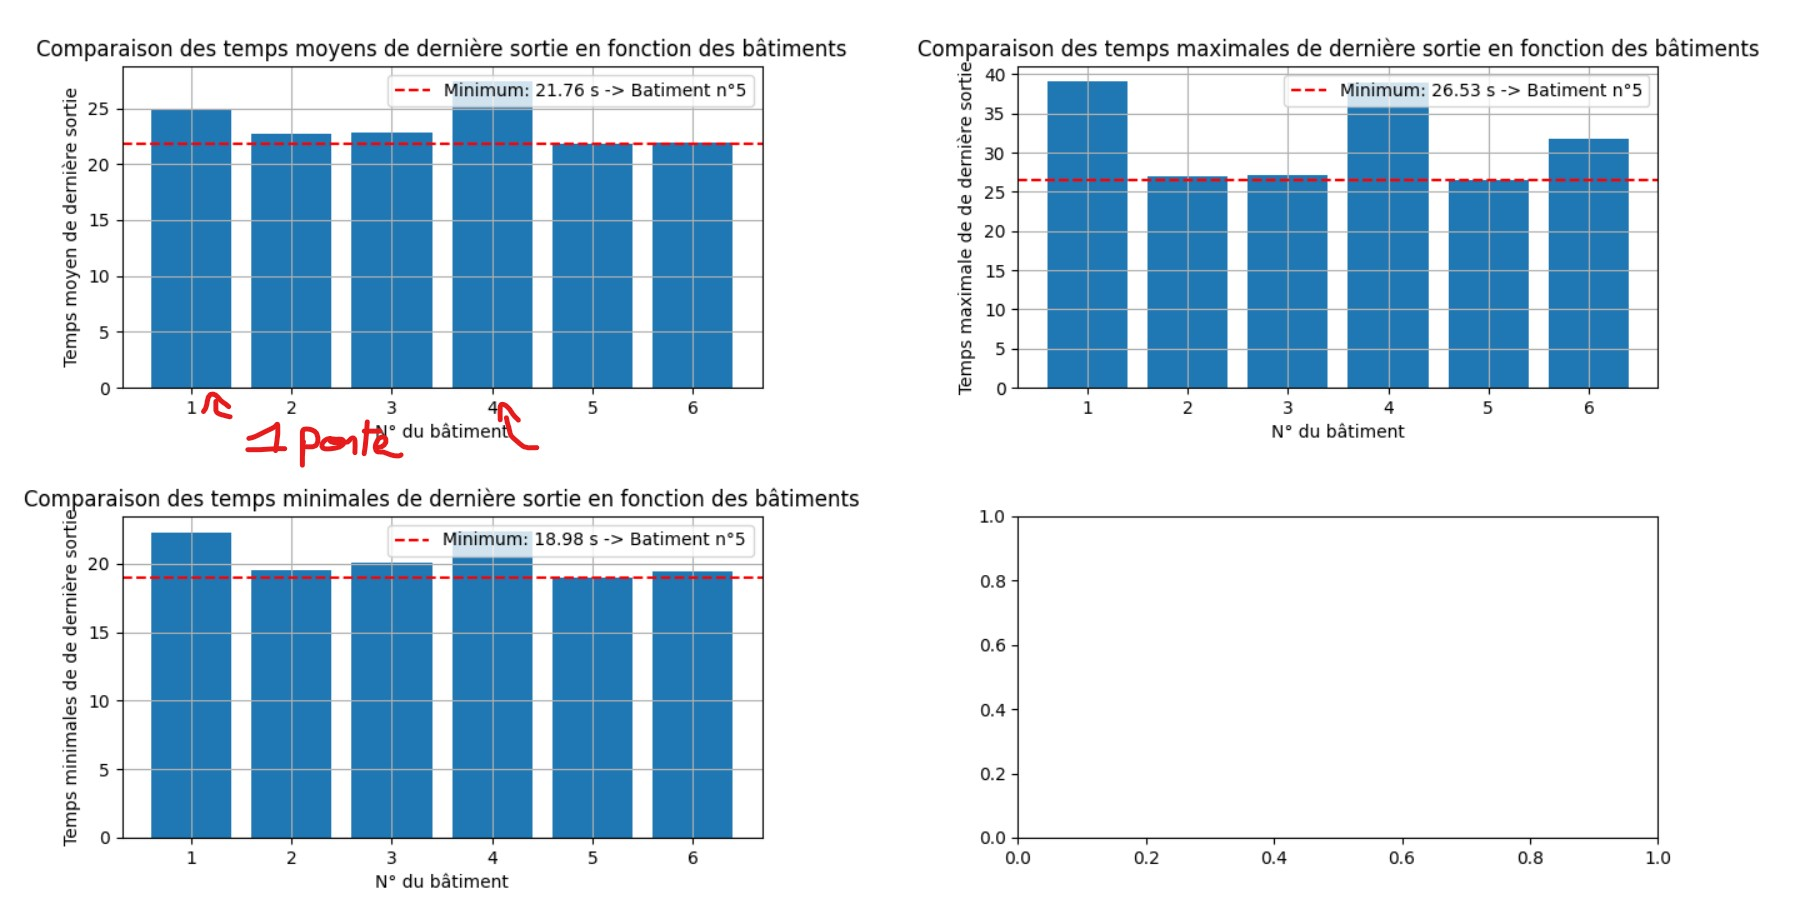
\includegraphics[scale=0.4]{3.(a) Resultat finaux.jpg}
\newline\newline


L'hypothèse de départ est validé, les bureaux proche du centre doivent effectivement avoir plusieurs portes, cela permet de créer de nouveaux chemins
et de fluidifier le trafic.
\newline\newline
Attention cependant, l'expérience montre qu'il ne faut pas qu'il y est trop de porte sinon les personnes tendent à emprunter un unique chemin ce qui créer des embouteillages,
ou des flux trop importants.
\end{document}